% !TeX spellcheck = ru_RU
% !TEX root = bfs_lodygin.tex

\section{Обзор}
\label{sec:relatedworks}
Для реализации алгоритма и необходимых для его работы компонентов не лишним будет для начала рассмотреть базовую теорию графов, ознакомиться с существующими методами хранения больших данных в памяти и иметь представление о многопоточном программировании.

\subsection{Терминология}
\textit{Граф} $\mathcal{G} = \langle V, E \rangle$~--- упорядоченная пара множеств, где $V$ конечное непустое множество вершин графа, а $E \subseteq V \times V$ множество рёбер. Рёбра графа могут обладать дополнительной информацией, в таком случае граф называется \textit{помеченным} и определятся тройкой $\langle V, E, L \rangle$, где $L$ это конечное множество меток графа. Под меткой стоит понимать данные, которые может содержать ребро в конкретной задаче. Например, если с помощью графа представлена карта, где города это вершины графа, а рёбра~--- дороги между городами, то в качестве меток могут быть взяты длины этих дорог.

\textit{Разреженный граф}~--- граф с малым количеством рёбер по отношению к количеству вершин.

Граф можно представлять в памяти как \textit{матрицу смежности}~--- квадратная матрица $M$ размеров $n \times n$, где $n$ это количество вершин в графе. Элементы такой матрицы $M[i,j]$ соответствуют единице, если между вершинами $i$ и $j$ существует ребро и нулю, если такое ребро отсутствует. В случае помеченного графа, элементы матрицы принимают вместо единицы значение метки, соответствующее данному ребру, а вместо нуля в матрице для обозначения отсутствия ребра, как правило, вводится специальное обозначение, например \texttt{None}.

\textit{Список рёбер}~--- другой подход к представлению графа в памяти. В списке рёбер в каждом узле записываются две смежные вершины и вес соединяющего 
их ребра (для помеченного графа).

\textit{Путь}~--- последовательность вершин, в которой каждая вершина соединена со следующей ребром.

Две вершины в графе считаются \textit{связными}, если между ними существует путь.

\textit{Дерево}~--- структура данных, состоящая из узлов, связанных между собой в виде иерархической структуры без циклов. Один из узлов в дереве называется корневым. Каждый узел может иметь ноль или более дочерних узлов. Узел, не имеющий дочерних узлов называется \textit{листом}.

\textit{Бинарное дерево}~---  это особый тип дерева, где каждый узел может иметь не более двух дочерних узлов.

\textit{Дерево квадрантов}~--- это дерево, в котором у каждого внутреннего узла ровно 4 потомка. Деревья квадрантов часто используются для рекурсивного разбиения двухмерного пространства по 4 квадранта (области).

\subsection{Представление графа в памяти}
Для хранения графа в памяти обычно используют матрицу смежности или список рёбер. При использовании матриц смежности в памяти создается двумерный массив, каждая ячейка которого соответствует элементу матрицы. Однако в случае малого количества рёбер в графе, такой подход нельзя считать рациональным, так как выделенная под несуществующие рёбра память расходуется впустую. При использовании списка рёбер проблема с избыточным использованием памяти решается, но возникают другие трудности, например, с добавлением новых рёбер или же с исследованием вершин на связность. Существует схожий со списком рёбер способ хранения в формате сжатой разреженной строки (\texttt{Compressed sparse row}), где матрица представляется тремя одномерными массивами, содержащими ненулевые значения, экстенты строк и индексы столбцов. Такой формат позволяет быстро обращаться к элементу по индексу и производить векторно-матричные операции, однако любое изменение графа в таком формате понесёт за собой большие накладные расходы, о чём говорится в статье Аапо Кироло~\cite{10.5555/2387880.2387884}.

Одним из решений данной проблем с избыточным использованием памяти является представление такой матрицы в виде дерева квадрантов (рисунок~\ref{fig:quadtree}), о чём в своей работе упоминает Гилберт~Дж.~Р.~\cite{bulucc2012parallel}. При таком подходе матрица рекурсивно разбивается на 4 части. В тот момент, когда в одной из частей отсутствуют значащие ячейки, разбиение останавливается и вся часть обозначается как незначащая. Преимуществом такой абстракции является не только сокращение объема памяти, требуемое для хранения графа, но и сохранение возможности применения векторно-матричных операций для реализации необходимых алгоритмов.

\begin{figure}[ht]
    \centering
    \incfig{quadtree}
    \caption{Представление матрицы в виде дерева квадрантов}
    \label{fig:quadtree}
\end{figure}

\subsection{Breadth-first search}
Обход в ширину~—-- один из простейших алгоритмов обхода графа, являющийся основой для многих важных алгоритмов для работы с графами. Он подразумевает поуровневое исследование графа:
\begin{enumerate}
\item  посещение одной или нескольких произвольно выбранных вершин;
\item  рекурсивное посещение всех смежных вершин для данной или данных.
\end{enumerate}
Вершины просматриваются в порядке возрастания кратчайшего пути до заданной. Алгоритм прекращает свою работу в случае обхода всех возможных вершин, либо в случае выполнения требуемого условия. Например, если задачей был поиск кратчайшего пути до определённой вершины. 

Данный алгоритм применяется для решения многих задач, одни из которых:
\begin{enumerate}
    \item  поиск кратчайшего пути;
    \item  поиск компонент связности;
    \item  поиск всех вершин/рёбер, лежащих на кратчайшем пути.
\end{enumerate}

Простейшей реализацией такого алгоритма является применение \textit{очереди}~--- абстрактного типа данных с дисциплиной доступа к элементам \enquote{первый пришёл --— первый вышел}. Первая вершина помещается в очередь с меткой $0$. Далее, рассматриваются все не посещенные ранее вершины, смежные с ней и добавляются в очередь с меткой данного шага алгоритма. Первая вершина удаляется из очереди и отмечается посещенной. Алгоритм продолжает работу, пока очередь не окажется пустой. Однако, существует другой подход к реализации данного алгоритма. Если граф представлен в виде матрицы смежности, то такой алгоритм возможно реализовать с помощью векторно-матричных операций линейной алгебры~\cite{davis2018algorithm}. Тогда алгоритм будет выглядеть следующим образом.
\begin{enumerate}
    \item  На вход поступает матрица смежности графа и вектор, в ячейках которого отмечены стартовые вершины.
    \item  Вектор (фронт) умножается на матрицу и на выходе получается вектор, в ячейках которого отмечены вершины, смежные с изначальными. Посещенные вершины заносятся в результирующий вектор.
    \item  Из фронта убираются все вершины, посещенные ранее. Предыдущий шаг повторяется.
    \item  Алгоритм завершает работу, когда вектор становится пустым.
\end{enumerate}

\begin{figure}[H]
    \centering
    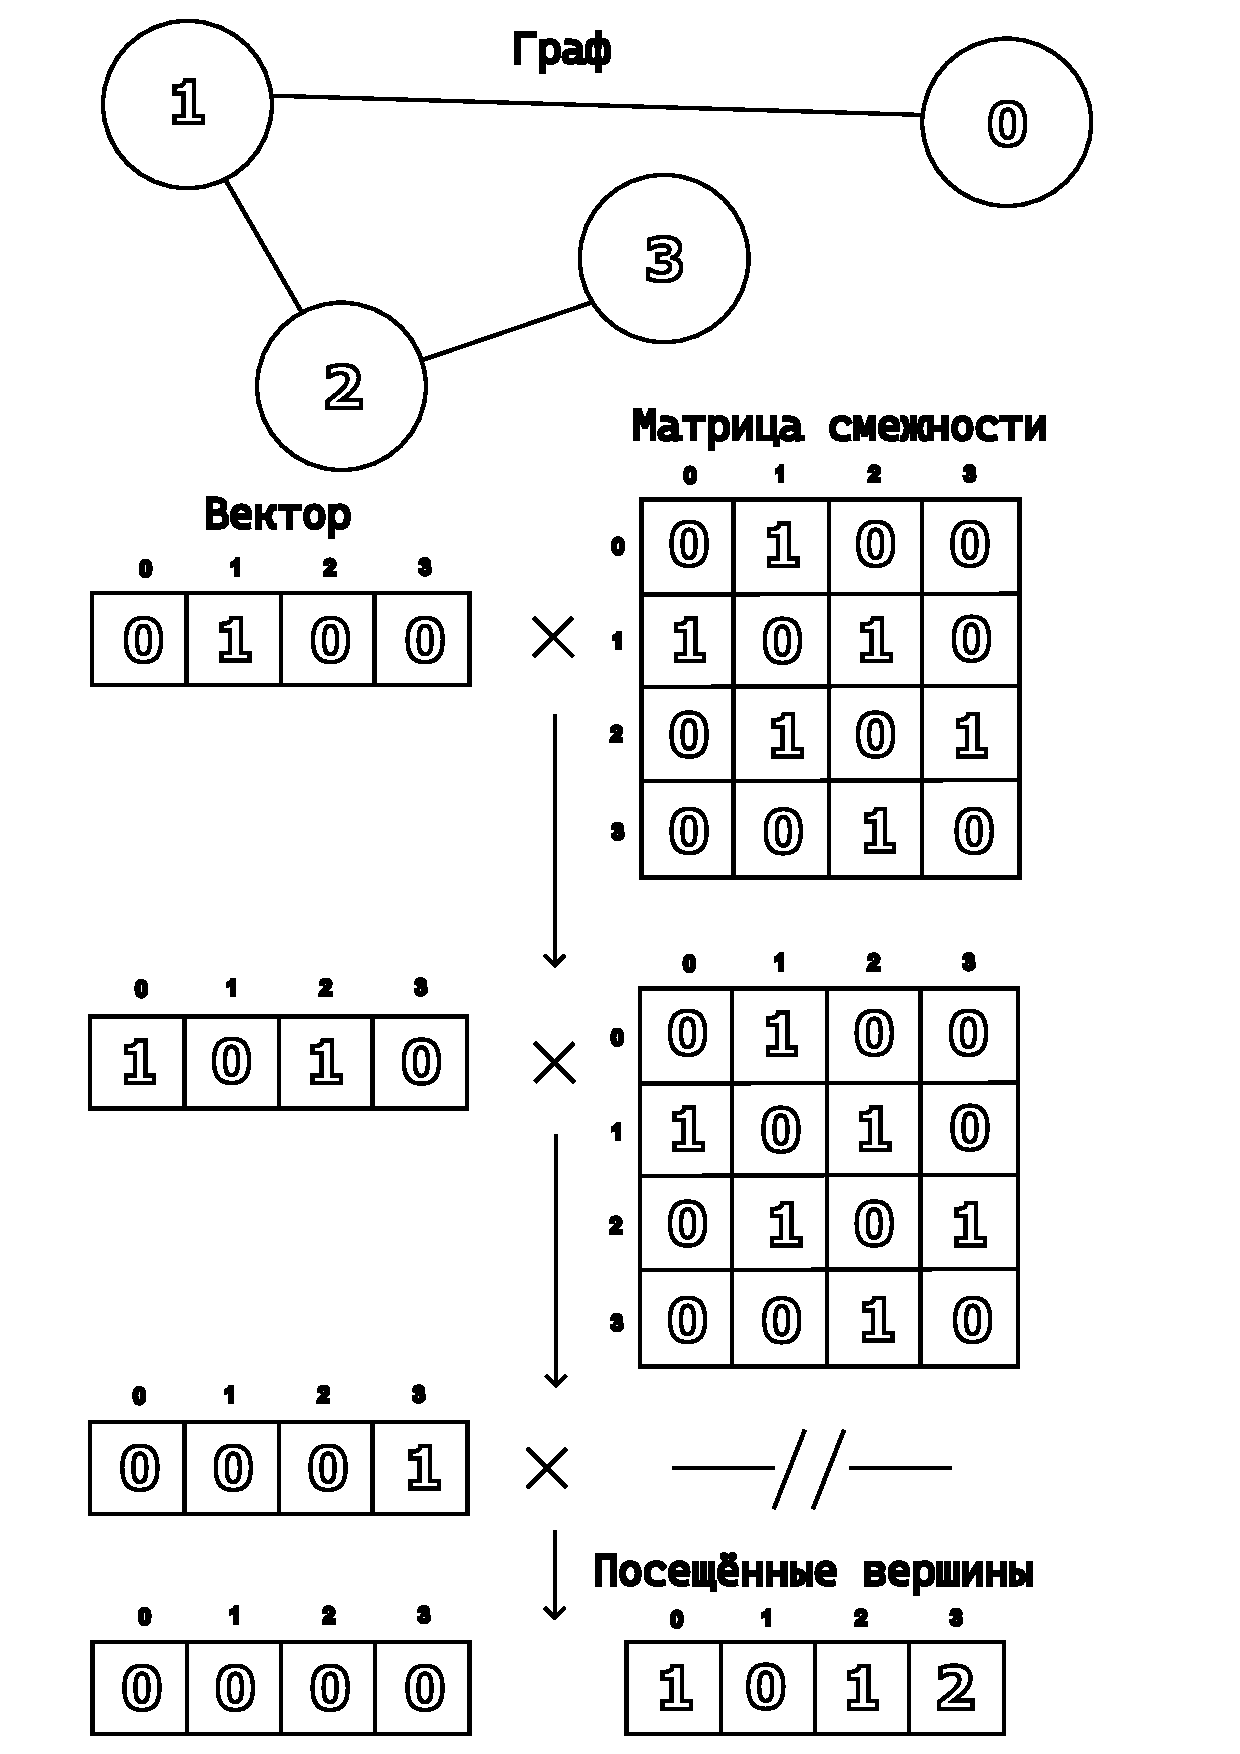
\includegraphics[width=\textwidth]{figures/linear_bfs.pdf}
    \caption{Алгоритм обхода в ширину с применением линейной алгебры}
    \label{fig:linearbfs}
\end{figure}

\subsection{Многопоточность}

\textit{Многопоточность}~--- это концепция, связанная с одновременным выполнением нескольких \textit{потоков} или нитей внутри одной программы. Потоки представляют собой последовательности инструкций, выполняющихся параллельно и независимо друг от друга, имея доступ к общим ресурсам программы. Многопоточные программы могут эффективно использовать многоядерные и многопроцессорные системы, что позволяет выполнять задачи параллельно и ускоряет выполнение программы. Однако такая концепция влечёт за собой ряд проблем. Во-первых, создание отдельного потока требует определённых ресурсов системы. При неумелом выделении количества потоков на решение задачи возможна потеря производительности, если накладные расходы на создание и \textit{синхронизацию} потоков превысят полученную выгоду от многопоточности. Во-вторых, при использовании общих ресурсов возникает риск \textit{состояния гонки} (race condition), когда несколько потоков пытаются одновременно изменять одни и те же данные. Это может привести к непредсказуемым результатам и ошибкам в программе. Наконец, многопоточность напрямую зависит от системы и её аппаратных возможностей. Количество \textit{ядер} и \textit{логических потоков} процессора однозначно определяют максимальное количество нитей, на которые следует разбивать нашу задачу во избежание потери производительности~\cite{Roberts2006MultiCorePI}.
%В обзоре необходимо ссылаться на работы других людей. В данном шаблоне задумано, что литература будет указываться в файле \verb=vkr.bib=. В нём указываются пункты литературы в формате \BibTeX{}, а затем на них можно ссылаться с помощью \verb=\cite{...}=. Та литература, на которую Вы сошлетесь, попадет в список литературы в конце документа. Если не сошлетесь~---  не попадёт. Спецификацию в формате \BibTeX{} почти никогда (для второго курса~--- никогда), не нужно придумывать руками. Правильно: находить в интернете описание цитируемой статьи\footnote{Например, \url{https://dl.acm.org/doi/10.1145/3408995} (дата доступа:   \DTMdate{2022-12-17}).},
%копировать цитату с помощью кнопки \foreignquote{english}{Export Citation} и вставлять в \BibTeX{} файл. Если так не делать, но оформление литературы будет обрастать багами.
%Например, \BibTeX{} по особенному обрабатывает точ\-ки, запятые и \verb=and= в списке авторов, что позволяет ему самому понимать, сколько авторов у статьи, и что там фамилия, что~--- имя, а что~--- отчество.

%В обзоре и в остальном тексте вы наверняка будете использовать названия продуктов или языков программирования. Для них рекоменду\-ется (в файле \verb=preamble2.tex=) за\-дать специальные команды, чтобы писать сложные названия правильно и одинаково по всему доку\-менту. Написать с ошибкой  название любимого языка программирова\-ния науч\-ного руко\-водителя~--- идеальный вариант его выбесить.
